Sometimes data structures include auxiliary fields that are useful for traversing the data structure
for debugging or diagnostic purposes. The presence of such fields, however can result in the more conservative shape.
To illustrate this we present the following example .

\section{Motivating Example}

\begin{example}
Consider the code segment in Program.~\ref{MotivatingExample} which has functions for searching data in a binary tree and 
inserting node into the same. The fields of structure {\tt Node}, which is used to realize the functions, are also shown. The 
structure {\tt Node} has three field pointers {\tt Left}, {\tt Right} and {\tt Parent}.
In the {\tt insert} function we can see a cycle getting created due to the lines {\tt S5} and {\tt S6}.
Take a look at Fig:~\ref{fig:Code} to see how the field sensitive analysis also
gets the shape of  \p  \ and  \s \ as a cycle at that point.

Now in the {\tt search} function, the {\tt Parent} pointer is
not at all used, so ideally the shape that is actually traversed inside the {\tt search} function is a Tree. But as the function is called
with the root of the tree, whose shape gets evaluated to Cycle in the {\tt insert} function,
we infer that the shape of the root as Cycle in the {\tt search} function as well even though the parent link is never been traversed. 
\end{example}
        
%  \begin{center}
% 
\begin{figure}
\begin{lstlisting}[caption={Motivating Example} ,label=MotivatingExample]
Struct Node {
  Struct Node *Left,*Right,*Parent;
  int key;
};
typedef Struct Node Node;

bool search(Node *root,int key){
if(root)
  return (key==root->key)||search(root->Left,key)||search(root->Right,key);
return 0;
}


void insert(Node *root,int key){
    Node *s=root;   //This pointer is used for traversing the Tree 
    ..
    //New node is inserted as a child of s(s can be any node of the tree)
    Node *p;
    S1. p=(Node *)malloc(sizeof(Node));    	
    S2. p->Left=NULL;			
    S3. p->Right=NULL;			
    S4. p->key=key;				
    S5. s->Left=p;				
    S6. p->Parent = s;			
    ..
}

\end{lstlisting}
\end{figure}

% \end{center}

\begin{figure}[h]
\centering
\begin{tabular}{@{}c@{}}

  \scalebox{0.80}{
    \begin{tabular}[b]{|c||c|c|}
          \hline 
          {\bf After} & $\Left_{p,t}$ & $\Parent_{t,p}$ \\ 
           \hline \hline
	  {\tt S1}       & false	  & false     \\ \hline
	  {\tt S2}       & false          & false     \\ \hline
	  {\tt S3}       & false 	  & false     \\ \hline
	  {\tt S5}       & true	          & false     \\ \hline
          {\tt S6}       & true	          & true     \\ \hline
    \end{tabular} 
      
  } \\
  \footnotesize (a) Boolean Variables  \\ \\
  

  \scalebox{0.80}{
\begin{tabular}[b]{|l@{}|@{}c@{}|@{}c@{}|} \hline
 {\bf After} & $D_F$ & $I_F$ \\ 
 {\bf Stmt} & & \\ \hline

{\tt S1} & 
\begin{tabular}{|p{3mm}|p{22mm}p{22mm}|} \hline 
            & $\p$  		& $\s$   \\ \hline
  $\p$ 	& $\epsilon$	& $\emptyset$	 \\ \hline
  $\s$ 	& $\emptyset$	& $\emptyset$	\\ \hline
\end{tabular}
 &
\begin{tabular}{|p{3mm}|p{45mm}p{45mm}|} \hline 
            & $\p$  		& $\s$   \\ \hline
  $\p$ 	& $\{(\epsilon,\epsilon)\}$	& $\emptyset$	 \\ \hline
  $\s$ 	& $\emptyset$	& $\emptyset$	\\ \hline
\end{tabular} \\ \hline

{\tt S2} & 
\begin{tabular}{|p{3mm}|p{22mm}p{22mm}|} \hline 
            & $\p$  		& $\s$   \\ \hline
  $\p$ 	& $\epsilon$	& $\emptyset$	 \\ \hline
  $\s$ 	& $\emptyset$	& $\emptyset$	\\ \hline
\end{tabular}
 &
\begin{tabular}{|p{3mm}|p{45mm}p{45mm}|} \hline 
            & $\p$  		& $\s$   \\ \hline
  $\p$ 	& $\{(\epsilon,\epsilon)\}$	& $\emptyset$	 \\ \hline
  $\s$ 	& $\emptyset$	& $\emptyset$	\\ \hline
\end{tabular} \\ \hline

{\tt S3} & 
\begin{tabular}{|p{3mm}|p{22mm}p{22mm}|} \hline 
            & $\p$  		& $\s$   \\ \hline
  $\p$ 	& $\epsilon$	& $\emptyset$	 \\ \hline
  $\s$ 	& $\emptyset$	& $\emptyset$	\\ \hline
\end{tabular}
 &
\begin{tabular}{|p{3mm}|p{45mm}p{45mm}|} \hline 
            & $\p$  		& $\s$   \\ \hline
  $\p$ 	& $\{(\epsilon,\epsilon)\}$	& $\emptyset$	 \\ \hline
  $\s$ 	& $\emptyset$	& $\emptyset$	\\ \hline
\end{tabular} \\ \hline

{\tt S5} & 
\begin{tabular}{|p{3mm}|p{22mm}p{22mm}|} \hline 
            & $\p$  		& $\s$   \\ \hline
  $\p$ 	& $\epsilon$	& $\emptyset$	 \\ \hline
  $\s$ 	& $\{\fieldD{Left}{}\}$	& $\emptyset$	\\ \hline
\end{tabular}
 &
\begin{tabular}{|p{3mm}|p{45mm}p{45mm}|} \hline 
            & $\p$  		& $\s$   \\ \hline
  $\p$ 	& $\{(\epsilon,\epsilon)\}$	& $\{( \epsilon,\fieldD{Left}{})\}$ 	 \\ \hline
  $\s$ 	& $\{(\fieldD{Left}{}, \epsilon)\}$	& $\emptyset$	\\ \hline
\end{tabular} \\ \hline

{\tt S6} & 
\begin{tabular}{|p{3mm}|p{22mm}p{22mm}|} \hline 
            & $\p$  		& $\s$   \\ \hline
  $\p$ 	& $\epsilon$	& $\{\fieldD{Parent}{}\}$	 \\ \hline
  $\s$ 	& $\{\fieldD{Left}{}\}$	& $\emptyset$	\\ \hline
\end{tabular}
 &
\begin{tabular}{|p{3mm}|p{45mm}p{45mm}|} \hline 
            & $\p$  		& $\s$   \\ \hline
  $\p$ 	& $\{(\epsilon,\epsilon)\}$	&  $\{( \epsilon,\fieldD{Left}{}),(\fieldD{Parent}{},\epsilon)\}$	 \\ \hline
  $\s$ 	& $\{(\fieldD{Left}{}, \epsilon),(\epsilon,\fieldD{Parent}{})\}$		& $\emptyset$	\\ \hline
\end{tabular} \\ \hline

\end{tabular} 

}  \\
 \footnotesize (b) Direction ($D_F$) and Interference ($I_F$) matrices  \\ \\
  


\scalebox{0.80}{
\begin{tabular}[b]{|c@{}|@{}c|}\hline
  Heap Pointer & Boolean Equations \\ \hline
{\tt $p_{cycle}$} & \{  ($\Parent_{p,s}  \wedge  False $) $\vee$ ($\Parent_{p,s} \wedge ( \num{D[s,p]} >= 1)$) \} $\vee$    \{ $\Left_{s,p}  \vee ( \num{D[p,s]} >= 1)$ \}  \\  \hline
{\tt $p_{dag}$} & \{ ($\Parent_{p,s} \wedge   ( \num{I[p,s]} > 1)$) \} \\ \hline 
{\tt $s_{cycle}$} & \{ $\Parent_{p,s} \wedge ( \num{D[s,p]} >= 1)$ \} $\vee$ \{  ($\Left_{s,p}  \wedge  False $) $\vee$ ($\Left_{s,p} \wedge   ( \num{D[p,s]} >= 1)$) \} \\ \hline
{\tt $s_{dag}$} & \{ ($\Left_{s,p} \wedge   ( \num{I[s,p]} > 1)$) \} \\ \hline
\end{tabular} 
} \\
\footnotesize (c) Boolean Equations after S6  \\    

\end{tabular}

\caption{Data Flow Values at each statement for Program.~\ref{MotivatingExample} }\label{fig:Code}
\end{figure}

For the above case, unlike the Field Sensitive Analysis, Subset Based Analysis can  identify the shape as Tree by considering the fields used by a 
function and using only those fields to infer the shape. Subset based analysis is a way in which only a subset of field pointers accessed in a 
function are used to get more precise shape information. We now present the details of the analysis.

\section{Analysis}    
The Field Sensitive Analysis needs to be modified slightly for the subset based analysis to occur.
During pre-processing of code, we parse each function separately and create a set of fields associated with each of them. This set will contain
all the field pointers that are used at least once in the function. We use $S_F$ to denote the subset of fields used by function \F.
For the functions present in  Program.~\ref{MotivatingExample}

\begin{center}
$S_{insert}$ = \{ Left , Right , Parent \} \\
$S_{search}$ = \{ Left , Right \} \\ 
\end{center}

During the evaluation of the boolean equations for function \F, we restrict our analysis to the fields that are present in $S_F$.
In this modified analysis when we reach a statement in \F\ we have to modify the evaluation of equations according to the following rules.

Any boolean equation would generally contain the  terms like $f_{\p\q}$,\ \DFM{\p}{\q},\ \IFM{\p}{\q}.
We replace each of the these terms by $f_{\p\q}^{\#} , {D^{\#}[p,q]} ,{I^{\#}[p,q]}$ respectively. Now lets 
understand what each of these terms mean.

\begin{itemize}

 \item $f_{\p,\q}^{\#}$ :
	  This term will have a value as False if  $\f$ is not accessed at any point in function \F, i.e $\f \not \in S_F$ 
If its present then the value is same as that of $f_{\p,\q}$
\begin{eqnarray*}
f_{\p,\q}^{\#} &=&  \left \{ \begin{array}{@{}ll}
                       f_{\p,\q}  & \f \in S_F  \\
			 \false & \mbox{Otherwise}
                       \end{array} \right.
\end{eqnarray*}

  \item ${D^{\#}[p,q]}$ :
      It contains the first field of all the paths that start from $\p$ and end at $\q$ except those whose first fields are not present in $S_F$.
In other way this is nothing but the difference of the contents of $D[p,q]$ and the set of all first fields for the paths from $\p$ to $\q$ whose
first fields are not present in $S_F$.

\begin{eqnarray*}
D^{\#}[\p, \q] &=& D[\p, \q] -\bigcup_{ \f \in \fields,\f \not \in S_F } \{  \project{D[\p,\q]}{f}         \}
\end{eqnarray*}

\item ${I^{\#}[p,q]}$ :
      Very similar to the way how $D^{\#}[\p, \q]$ was defined this term is also defined.      
\begin{eqnarray*}
I^{\#}[\p, \q] &=& I[\p, \q] - \bigcup_{ \f \in \fields,\f \not \in S_F } \{  \project{I[\p,\q]}{f}         \}
\end{eqnarray*}
\end{itemize}

After making all these replacements we evaluate the equation to get the shape.
Now that we have all the details about the analysis, lets look at how it works for the above mentioned motivating example.

% small code snippet present in Fig.~\ref{fig:SampleCode_Info}(a).

\begin{example}
 The function {\tt search} would be called with the root of the Tree as the parameter.
In Program.~\ref{MotivatingExample} that the variable {\tt root} is assigned to {\tt s} in the insert function. So at the end of the
insert function whatever boolean equation {\tt s} would have, {\tt root} also would have the same except replacing every {\tt s} by {\tt root} in the equation.
Actually the insert function may be recursive or iterative, if we consider the equation of {\tt s} at the end of complete insert function
it would be very large and explaining would be a lot difficult. So we have considered the equation only at the end of statement {\tt S6}. 
From Fig:~\ref{fig:Code}(c). the the boolean equation of {\tt root} is derived as 
\begin{eqnarray*}
{\tt root_{cycle}} &=& \{ \Parent_{p,root} \wedge ( \num{D[root,p]} >= 1) \} \vee \{  (\Left_{root,p}  \wedge False) \vee \\
 && (\Left_{root,p} \wedge   ( \num{D[p,root]} >= 1)) \} \\
{\tt root_{dag}} &=&  \{ (\Left_{root,p} \wedge   ( \num{I[root,p]} > 1)) \} 
\end{eqnarray*}

Even with the dataflow values concerning the Boolean variables, Direction and Interference matrices, {\tt root} would have the same values corresponding to that
of {\tt s} at the end of statement {\tt S6}. Hence at the start of  {\tt search} function $\Left_{root,p} = \true , \Parent_{p,root} = \true$  while the matrices are as given below.  \\

\scalebox{0.80}{
\begin{tabular}[b]{|@{}c@{}|@{}c@{}|} \hline
\begin{tabular}{|p{6mm}|p{22mm}p{22mm}|} \hline 
   D         & $\p$  		& $root$   \\ \hline
  $\p$ 	& $\epsilon$	& $\{\fieldD{Parent}{}\}$	 \\ \hline
  $root$ 	& $\{\fieldD{Left}{}\}$	& $\emptyset$	\\ \hline
\end{tabular}
 &
\begin{tabular}{|p{6mm}|p{45mm}p{45mm}|} \hline 
   I         & $\p$  		& $root$   \\ \hline
  $\p$ 	& $\{(\epsilon,\epsilon)\}$	&  $\{( \epsilon,\fieldD{Left}{}),(\fieldD{Parent}{},\epsilon)\}$	 \\ \hline
  $root$ 	& $\{(\fieldD{Left}{}, \epsilon),(\epsilon,\fieldD{Parent}{})\}$		& $\emptyset$	\\ \hline
\end{tabular} \\ \hline
\end{tabular} 
}

\par
Before going into the search function we need to know the small change this function undergoes when represented in intermediate form(GIMPLE) on which the
analysis takes place. The function would transform to

\begin{figure}[h]
\begin{lstlisting}
bool search(Node *root,int key){
       Node *temp1,*temp2;
       int tempInt;
St1:   temp1=root->left;
St2:   temp2=root->right;
       tempInt=root->key
       if(root)
         return (key==tempInt)||search(tmep1,key)||search(temp2,key);
       return 0;
}
\end{lstlisting}
\end{figure}

At the statement {\tt St1} first time the boolean equation will be evaluated for this function. We are not considering the evaluation after {\tt St2} because it would be done in the same way as that of {\tt St1}. 
As $\GenC{temp1} = \InC{root}$ and $\KillC{temp1} = \InC{temp1}$,  
$\OutC{temp1}$ is same as $\InC{root}$. Now lets look at each term in $\InC{root}$ and find what it evaluates to in the subset based analysis. 
\begin{eqnarray*}
 Parent_{p,root}^{\#} &=& \false  \ \ \ (Parent \not \in S_{Search} ) \\
 Left_{root,p}^{\#} &=& Left_{root,p} \  (Left \in S_{Search} ) \\
 D^{\#}[root,p] &=& D[root,p] - \project{D[root,p]}{Parent} \\
		&=& D[root,p] - \phi \\
		&=& \{\fieldD{Left}{}\} \\
 D^{\#}[p,root] &=& D[p,root] - \project{D[p,root]}{Parent} \\
		&=& D[p,root] - \{\fieldD{Parent}{}\} \\
		&=& \phi
\end{eqnarray*}

Substituting these above values in the equation of $\InC{root}$ would result in $\false$. In the similar way when we try to evaluate $\InD{root}$ it would give us $\false$, thus rightly detecting the shape of data structure traversed
as Tree.
\end{example}

\par
Note that the subset based analysis increases the precision at the cost of extra computation required to compute $D^{\#} ,I^{\#}$ and $f^{\#}$.
Due to the lack of sufficient benchmarks its not very clear to us if and when this overhead can be threat by the gain in precision. More work is required to evaluate this trade off.


% {\red
% \section{Limitations}
% In the Field sensitive analysis only the first field information in a path between two labelled nodes are present in the matrices, and 
% we are using that information in our subset based analysis. But this information is not always sufficient to get the exact shape 
% (considering the fields accessed in a function).To get the accurate results the information about the set of all fields that are being used in a path 
% is required or in other way we need the complete information about the heap graph. As this is very difficult to gather
% so we will end up with less precise (but conservative) results. We present one such example of safe result.
% \begin{example}
% Consider the heap graph in Fig.~\ref{Subset_fig}. This heap graph contains 3 unlabeled nodes and 2 labeled nodes. Assume that the solid edges are 
% constructed in {\tt main} function and the dotted edge is the last one to be constructed in some function {\tt foo} called from {\tt main}. Also assume 
% that in the {\tt foo} function, field $\f$ is the only one that is accessed.
% When the statement $Q \rightarrow \f = P$ is encountered in {\tt foo} the following data flow boolean equation is generated.
% \begin{eqnarray*}
% \GenC{Q}   &=&  (f_{QP} \wedge \InC{P}) \vee (f_{QP} \wedge (\num{\DFM{P}{Q}} \geq 1)) 
% \end{eqnarray*}
% In the second term of the above disjunction, the value of the cell  $\DFM{P}{Q}$ would be  $\{ \fieldI{f}{}{1} \}$ as there is only one path from $P$ 
% to $Q$ and it starts by field $\f$. No information is available about the presence of $\g$ field in that path, and $D^{\#}[P,Q]$ evaluates 
% to $\{ \fieldI{f}{}{1} \}$ making the value of $\GenC{Q}$ as TRUE. So even though in the function the field $\g$ is not accessed, but
% a cycle is formed using that field we are reporting it as a cycle.
% \end{example}
% 
% \begin{figure}[h]
% \centering
% \begin{tabular}{c}
%  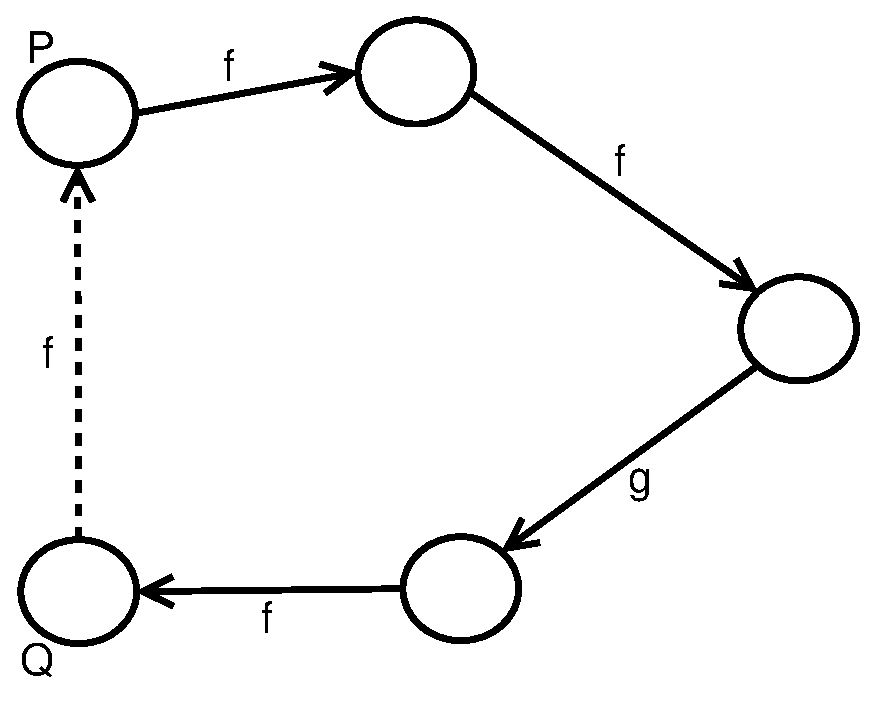
\includegraphics[scale=.3]{diagrams/Subset_11.eps} 
% \end{tabular}
% \caption{heap graph} \label{Subset_fig} 
% \end{figure}
% 
% }
% 
